\section{Introduction}
\label{sec:Introduction}


Digital multi-scale maps such as Google Maps and OpenStreetMap 
support zooming by displaying maps at different levels. 
This discrete strategy may results in sudden changes, which disturb user navigation.
To provide better zooming experience, 
we try to produce a sequence of maps 
with small incremental changes from a level to another level.
This process is known as \emph{continuous generalization}.

A way to achieve continuous generalization is to use morphing.
Often, a start map and a goal map, 
respectively at a larger scale and a smaller scale, 
are used as input, 
then maps at intermediate scales are produced 
while the start map is morphed to the goal map.
In order to morph, correspondences between two maps need to be defined.
For example, corresponding points between a pair of polylines have been 
investigated based on 
dynamic programming \citep{mnwb-mpstc-08}, 
Delaunay triangulations and binary line generalized tree (BLG-tree)  
\citep{Deng2015},
and simulated annealing \citep{Li2017_Annealing}.
From a point to its corresponding point,
a straight-line trajectory is often used to interpolate.
Using morphing, \citet{Peng2016_Admin} continuously generalized 
administrative boundaries based on compatible triangulations. When the number of line features is different in the start and goal maps, a continuous selection is required and \citet{Chimani2014_Eat} proposed to generate a selection sequence applicable for road network.
They removed one road at each step while keeping the remaining roads connected.

These methods are interesting but only work on lines and our problem of building polygon interpolation cannot be achieved by similar morphings. Regarding the continuous generalization of polygon map features,
\citet{Danciger2009} proposed to grow polygons when a map was zoomed out. Their method 
preserves polygons' topology, area-ratios, and relative positions.  In the case where the goal map is an aggregated version of start landcover map, \citet{Peng2017_AStar} computed optimal aggregation sequences for land-cover areas.

Buildings are important elements on maps, many methods have been proposed to generalize them but not necessarily in a continuous way.
For example, \citet{haunertwolff2010} simplified a set of buildings 
based an integer program.
Their simplification minimizes the number of edges of all the buildings 
and guarantees that the errors are smaller than a user-defined tolerance.
At the same time, no topological conflict is introduced by the simplification.
\citet{Buchin2011_Simp} simplified buildings based on an edge-move operation.
One advantage is that their method preserves orientations of the edges.

When users zoom out on digital maps, 
buildings become smaller and the distances between buildings decrease. So simplification is not the only necessary operation, and buildings can also be aggregated to legible enough \cite{Weibel1997}. Several methods were proposed to aggregate buildings while preserving the shape of buildings (right angles remain) \cite{Regnauld2001}, \cite{RegnauldRevell07}, \cite{Damen2008}. These algorithms can be used as inspirations to define a continuous transformation of buildings.

Algorithms were also proposed to create built-up area polygons (that appear in our goal map) from individual building polygons (that appear in our start map). For instance, \citet{Chaudhry2008} identified the boundaries of urban settlement by calculating `citiness' based on buildings. But the method cannot be adapted to provide a continuous transformation from the buildings to the built-up area.

Finally, some papers directly tackle the continuous transformation of buildings when scale is reduced. \citet{Li2017_Building} morphed between two buildings at different scales.
They managed to preserve the orthogonal characteristics of buildings, but their algorithm cannot be used in our case as the goal map does not contain buildings anymore. \citet{Touya17b} proposed a progressive transformation of buildings into a built-up area, where buildings are progressively replaced by the shape of the block they belong to. However, this last algorithm is not continuous enough, as each iteration directly transforms a set of buildings in a block into a polygon that covers the whole block. So there is no existing solution for the continuous generalization of building polygons into built-up area polygons.


Our contributions are as follows.
In \sect\ref{sec:Methodology},
we continuously generalize a start map, of buildings, 
to a smaller-scale goal map.
The generalization consists of aggregating, growing, and simplifying.
We aggregate original buildings which will be too close at an output scale 
by introducing bridges.
We grow (bridged) original buildings by buffering,
where we use so-called \emph{miter} joins to keep the right angles of buildings.
Because of using this kind of joins instead of \emph{round} ones,
we have more problems.
We show how to solve these problems.
We also simplify the buildings at the output scale.
We carry out a case study 
and discuss the performances of our method in \sect\ref{sec:CaseStudy}.
We conclude our paper in \sect\ref{sec:Conclusion}.



\section{Methodology}
\label{sec:Methodology}
We name our input map as start map,
and denote the scale of the start map by $1:M_\mathrm{s}$.
We generate a goal map at scale $1:M_\mathrm{g}$ 
($M_\mathrm{g} > M_\mathrm{s}$) by generalizing the start map. 
We use time $t\in[0,1]$ to define the continuous generalization
process. 
We require that the generalization yields exactly the start map when $t=0$ 
and the goal map when $t=1$.
The start map should be continuously changed to the goal map 
when $t$ increases from~$0$ to~$1$.
For the sake of convenience, we define parameter
$M_t= M_\mathrm{s} + t \cdot (M_\mathrm{g}-M_\mathrm{s})$.

We group buildings which will be too close at time $t$
and aggregate the buildings in the same group by introducing bridges.
We grow the buildings by buffering with miter joins.
Our building simplification consists of two steps.
The first one is to use dilation and erosion to remove pits and spikes.
The second step is to remove vertices using Imai--Iri algorithm.
To make sure that the intermediate-scale buildings never shrink,
we merge the shape of a building with the shape at the previously immediate 
step. 
Also, we clip the building using the shape on goal map.


\subsection{Grouping buildings based on buffering}
\label{sec:Group}
There are many ways to group buildings.

Using MST to group buildings: \citet{Zhang2013, 
	Cetinkaya2015,Deng2017,Regnauld1996}


We group buildings based on their buffers
(see \fig\ref{fig:RemoveBay} for example).
We wish to remove some ``bays'' 
which have widths less than $2 \dtrm{D}$.
A bay may appear after some buildings are merged by bridging
(see for example \fig\ref{fig:RemoveBay}e).
To remove such kind of bay,
we overgrow (see \fig\ref{fig:RemoveBay}b and~e) 
and then erode back (see \fig\ref{fig:RemoveBay}c and~f) 
with distance $\dtrm{D}$.
There may be some buildings in a bay (see \fig\ref{fig:RemoveBay}c),
so we iteratively group until the number of groups does not decrease.
The result of having removed a bay is the outer polygon of 
\fig\ref{fig:RemoveBay}h. 
In comparison, the result is \fig\ref{fig:RemoveBay}e 
if we do not remove a bay.
Note that the pit we want to remove in \fig\ref{fig:RemovePitAndSpike} is a 
kind of bay and will be removed by overgrowing.


\begin{figure*}[tb]
	\centering
	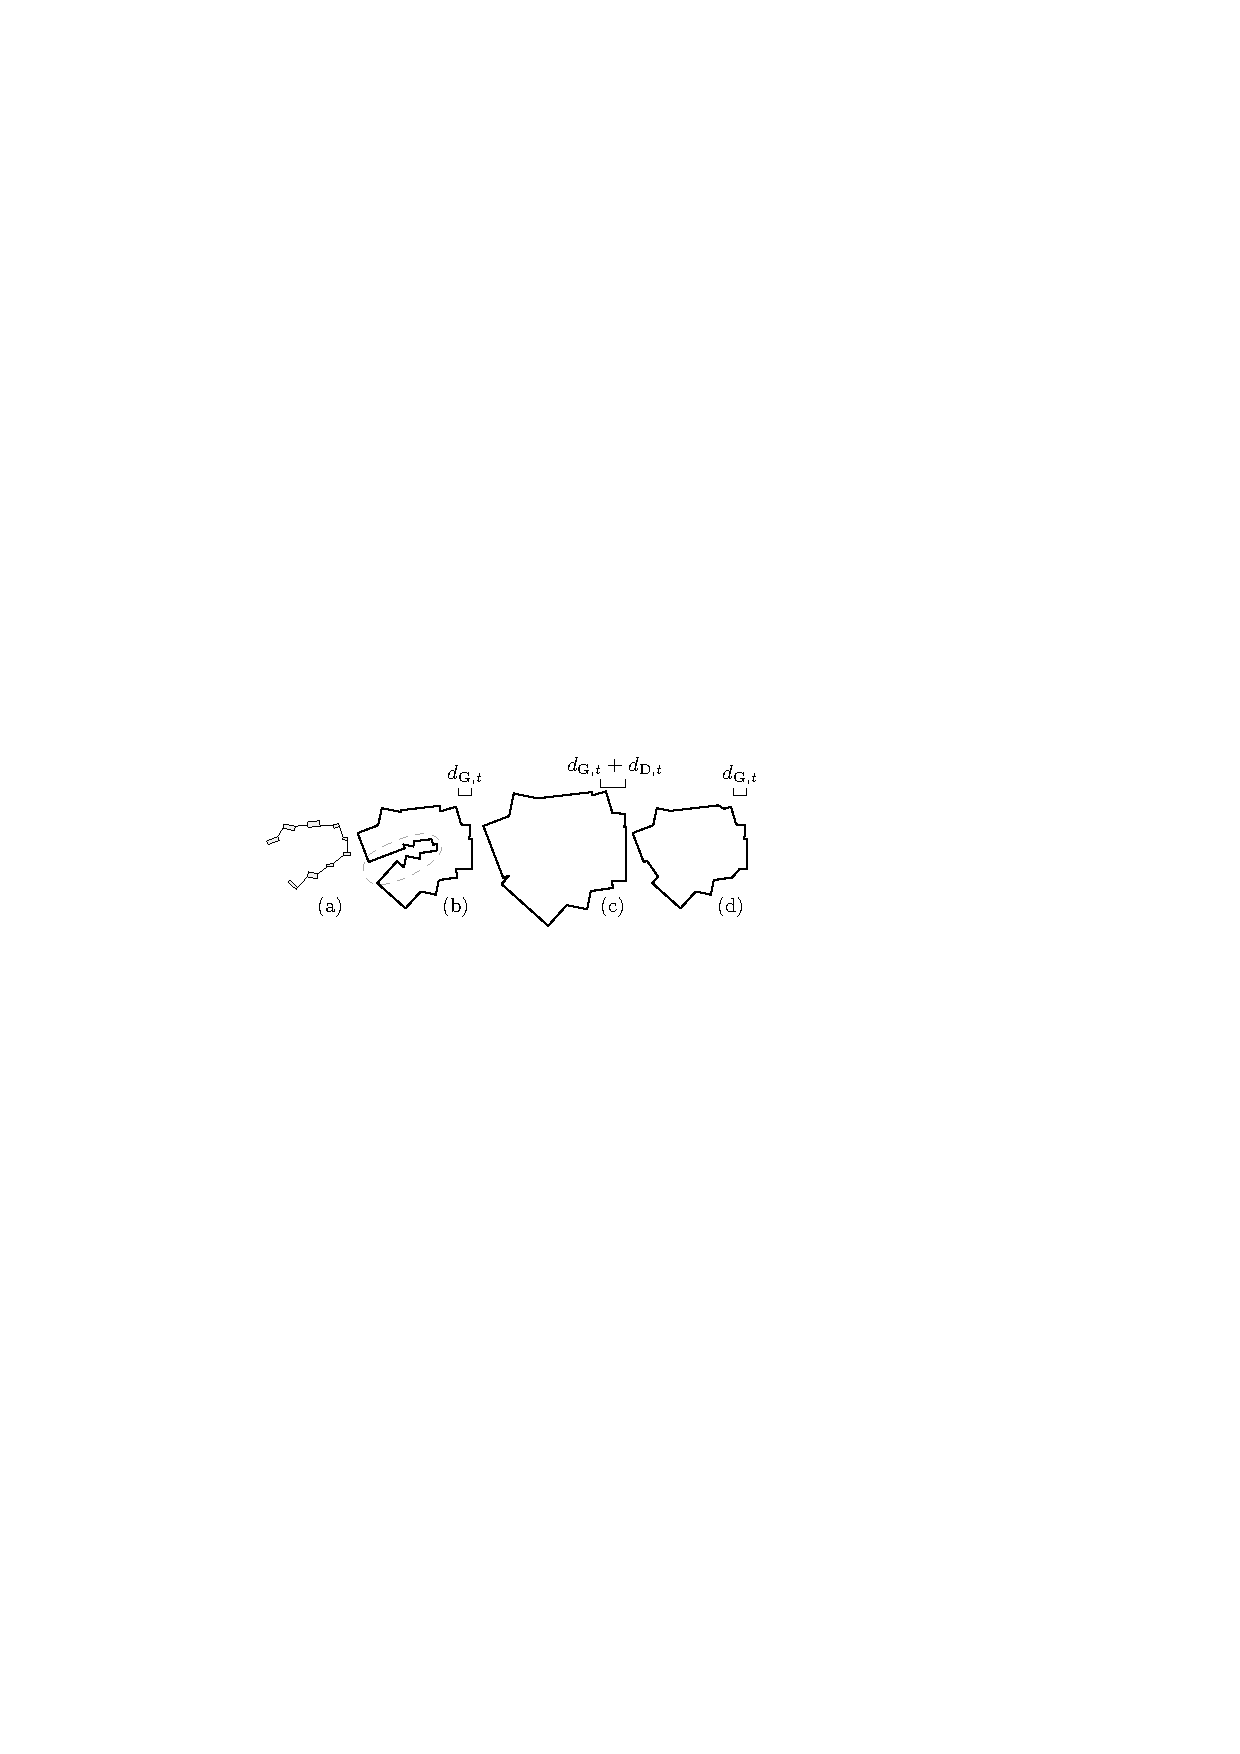
\includegraphics[draft=false]{RemoveBay}
	\caption{Group buildings iteratively.
		(a) Original buildings.
		(b) Dilate each building in (a) with distance $\dtrm{G}+\dtrm{D}$.		
		(c) Erode the polygons in (b) with distance $\dtrm{D}$.
		(d) Dilate the polygons in (c) with distance 
		$\frac{\sqrt{5}}{2} d_{\epsilon,t}$. 
		If two polygons in (d) intersect, 
		the original buildings in (a) will be put in the same group 
		because they will become too close at time $t$.
		Until this step, there two groups according to (d), 
		one consists of the single middle building and 
		the other group consists of the surrounding $9$ buildings.
		(e) The result of growing and merging at time $t$ 
		if we use $\dtrm{D}=0$.
		The process of (f), (g), and (h) is similar to 
		that of (b), (c), and (d).		
		The difference is that 
		instead of applying the operators to each single building, 
		we do that for the buildings in the same group.
		In (f), we manage to remove the bay in (e) by additionally dilating 
		with distance $\dtrm{D}$.
		There is only one group left according to (h).
		We iteratively group buildings in this way until the number of groups 
		does not decrease.
	}
	%in this example, we used _dblTotalGrow *= 5;
	\label{fig:RemoveBay}
\end{figure*}




\subsection{Aggregating close buildings by introducing bridges}
\label{sec:Merge}
The distance between two buildings on a map should be larger than a threshold
\citep{Regnauld2001,Li2004}.
Following \citet{Basaraner2008,Stoter2009}, 
we set the separation threshold $\epsilon= 0.2\,\mathrm{mm}$. 
The real separation distance at time $t$ is
\begin{equation}
	\label{eq:d_epsilont}
	d_{\epsilon, t} = \epsilon \cdot M_t.
\end{equation}

If a group of buildings become too close during growing,
we merge them by introducing bridges (see \fig\ref{fig:GrowAndBridge}).
We will talk about where to add bridges in \sect\ref{sec:Goal}.
No matter a bridge appear earlier or later, 
it has width $2\dtrm{G}$ at time $t$.
This setting guarantees that no bridge is thin when $t=1$.
For example, the two bridges in \fig\ref{fig:GrowAndBridge} at time $t=1$ have 
the same widths.
This setting is achieved by following.
We detect nearest points for each pair of buildings at time $t=0$ so that 
we know where we should add bridges.
At time $t$, we group buildings that are too close to each other,
then we merge them by adding the precomputed bridges.
For this merged building, we grow, simplify, and unite as described in 
\sects\ref{sec:Grow}, \ref{sec:Simplify}, and~\ref{sec:Unite}.
We may unite the processed merged building with several separate parts 
because the group of buildings may be in several smaller groups
in the immediately previous step.

\todo[inline]{actually larger than $d_{\epsilon, t}$.}


\begin{figure*}[tb]
	\centering
	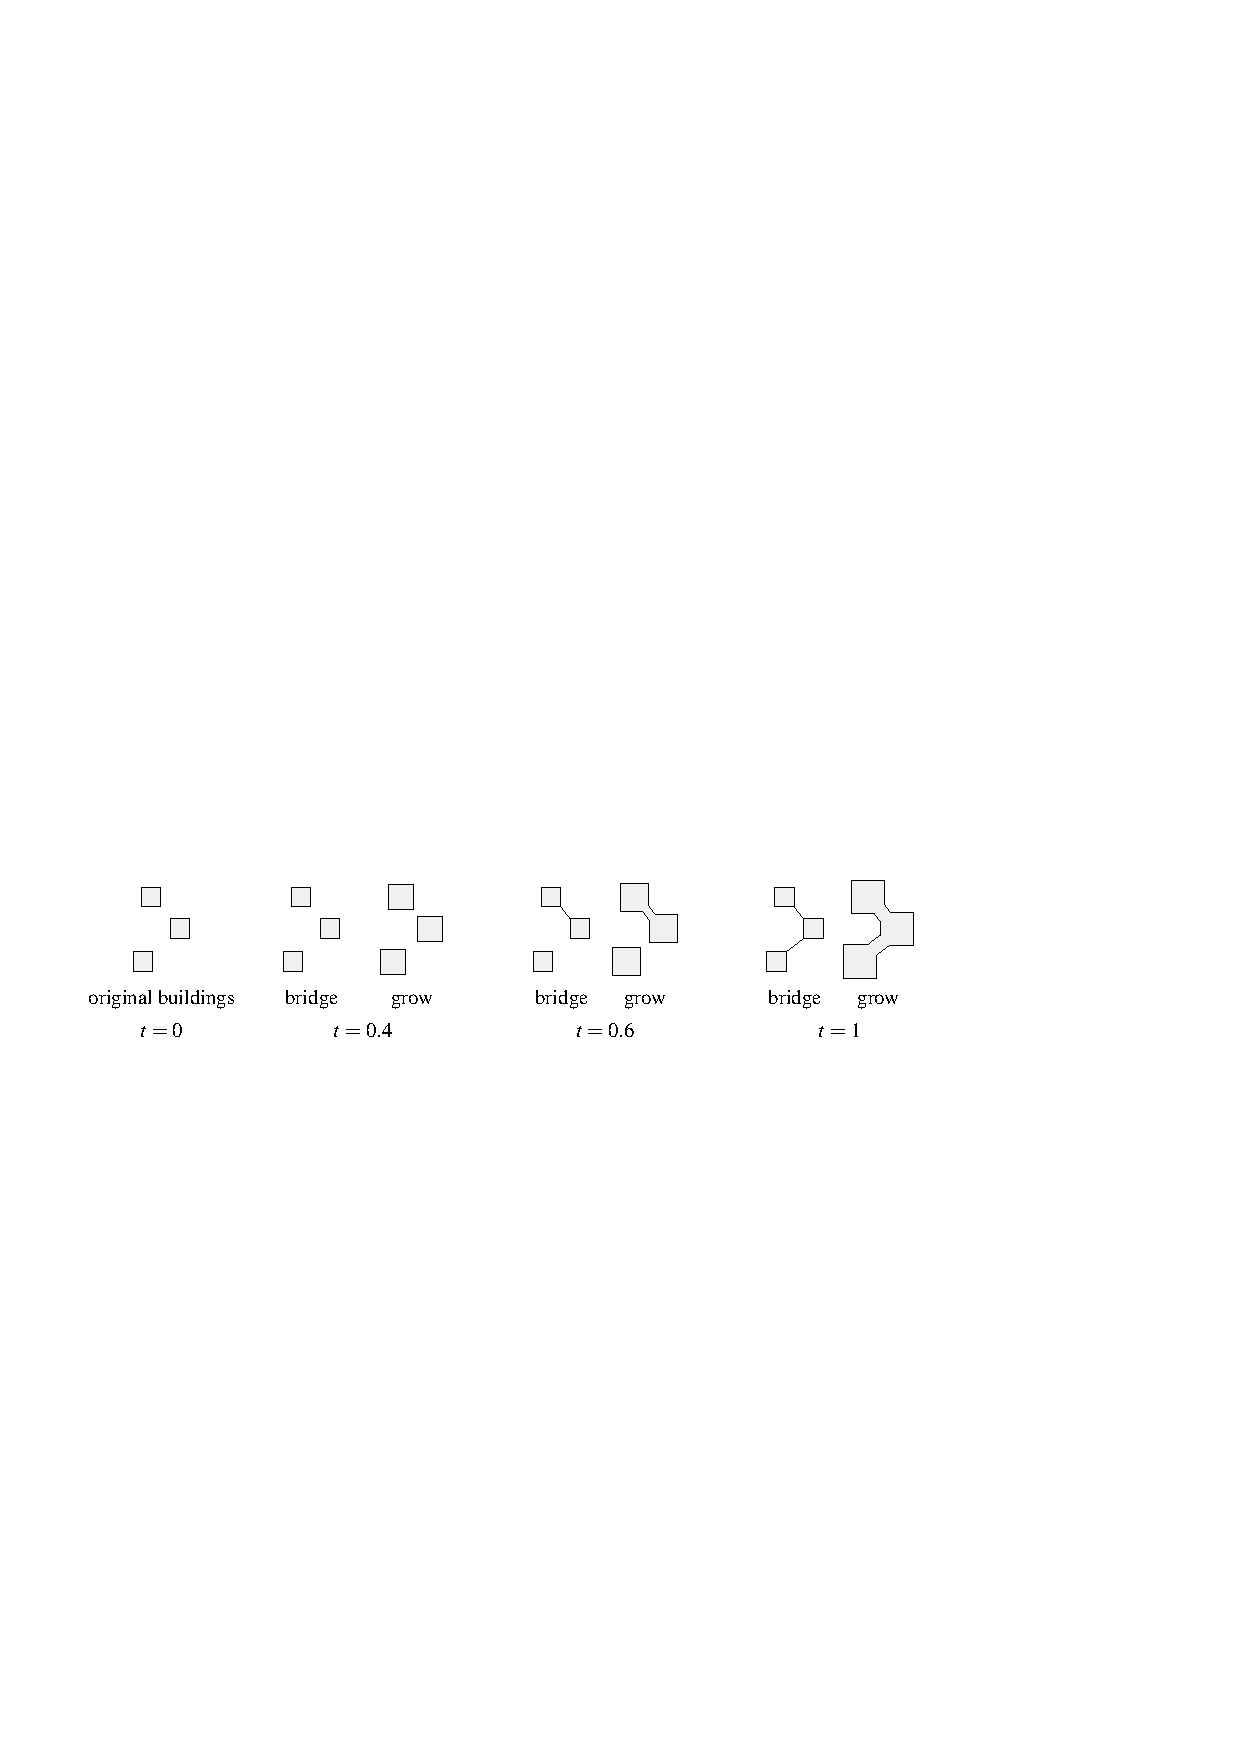
\includegraphics[draft=false]{GrowAndBridge}
	\caption{Merge buildings by introducing bridges when the buildings become 
		too close.
		Although the bridges appear at different time, 
		their widths are the same (see the figure with $t=1$).}
	\label{fig:GrowAndBridge}
\end{figure*}

For each pair of buildings in the same group, 
we find the smallest distance between them.
We connect the buildings by adding an edge from the nearest points.
We find a minimum spanning tree of the buildings using Prim's algorithm 
\citep{Prim1957}.
We enlarge and merge buildings as the way we do in \sect\ref{sec:Group}.

\subsection{Growing buildings based on buffering}
\label{sec:Grow}
We grow building based on buffering. 
There are two typical ways of buffering polygons, i.e.,
one with round joins and the other with miter joins 
(see \fig\ref{fig:Buffer_TwoKinds}).
As buildings are usually rectangles, 
we choose the second way because it is 
better at keeping the right angles.
If an angle is acute, however, an excessively long \emph{spike} will be 
produced.
This spike may go across other buildings 
(see \fig\ref{fig:Buffer_MiterLimits}a).
To avoid this kind of interruptions, 
we require that for an angle if a vertex of the 
buffer is more than $\alpha d_\mathrm{G} (\alpha \ge 1)$, 
where $d_\mathrm{G}$ is the growing distance, 
away from the original vertex, 
a \emph{square} joining is applied
(see \fig\ref{fig:Buffer_MiterLimits}b).
To keep right angles of buildings, 
we must have $\alpha \geq \sqrt{2}$. 
We set $\alpha  = 1.5$ so that a square joining is applied when an angle is 
smaller (more acute) than $83.6 \degree$.

\begin{figure}[tb]
	\centering
	
\includegraphics{Buffer_TwoKinds}
	\caption{Buffering a polygon using different kinds of joins.}
	\label{fig:Buffer_TwoKinds}
\end{figure}

\begin{figure}[tb]
	\centering
	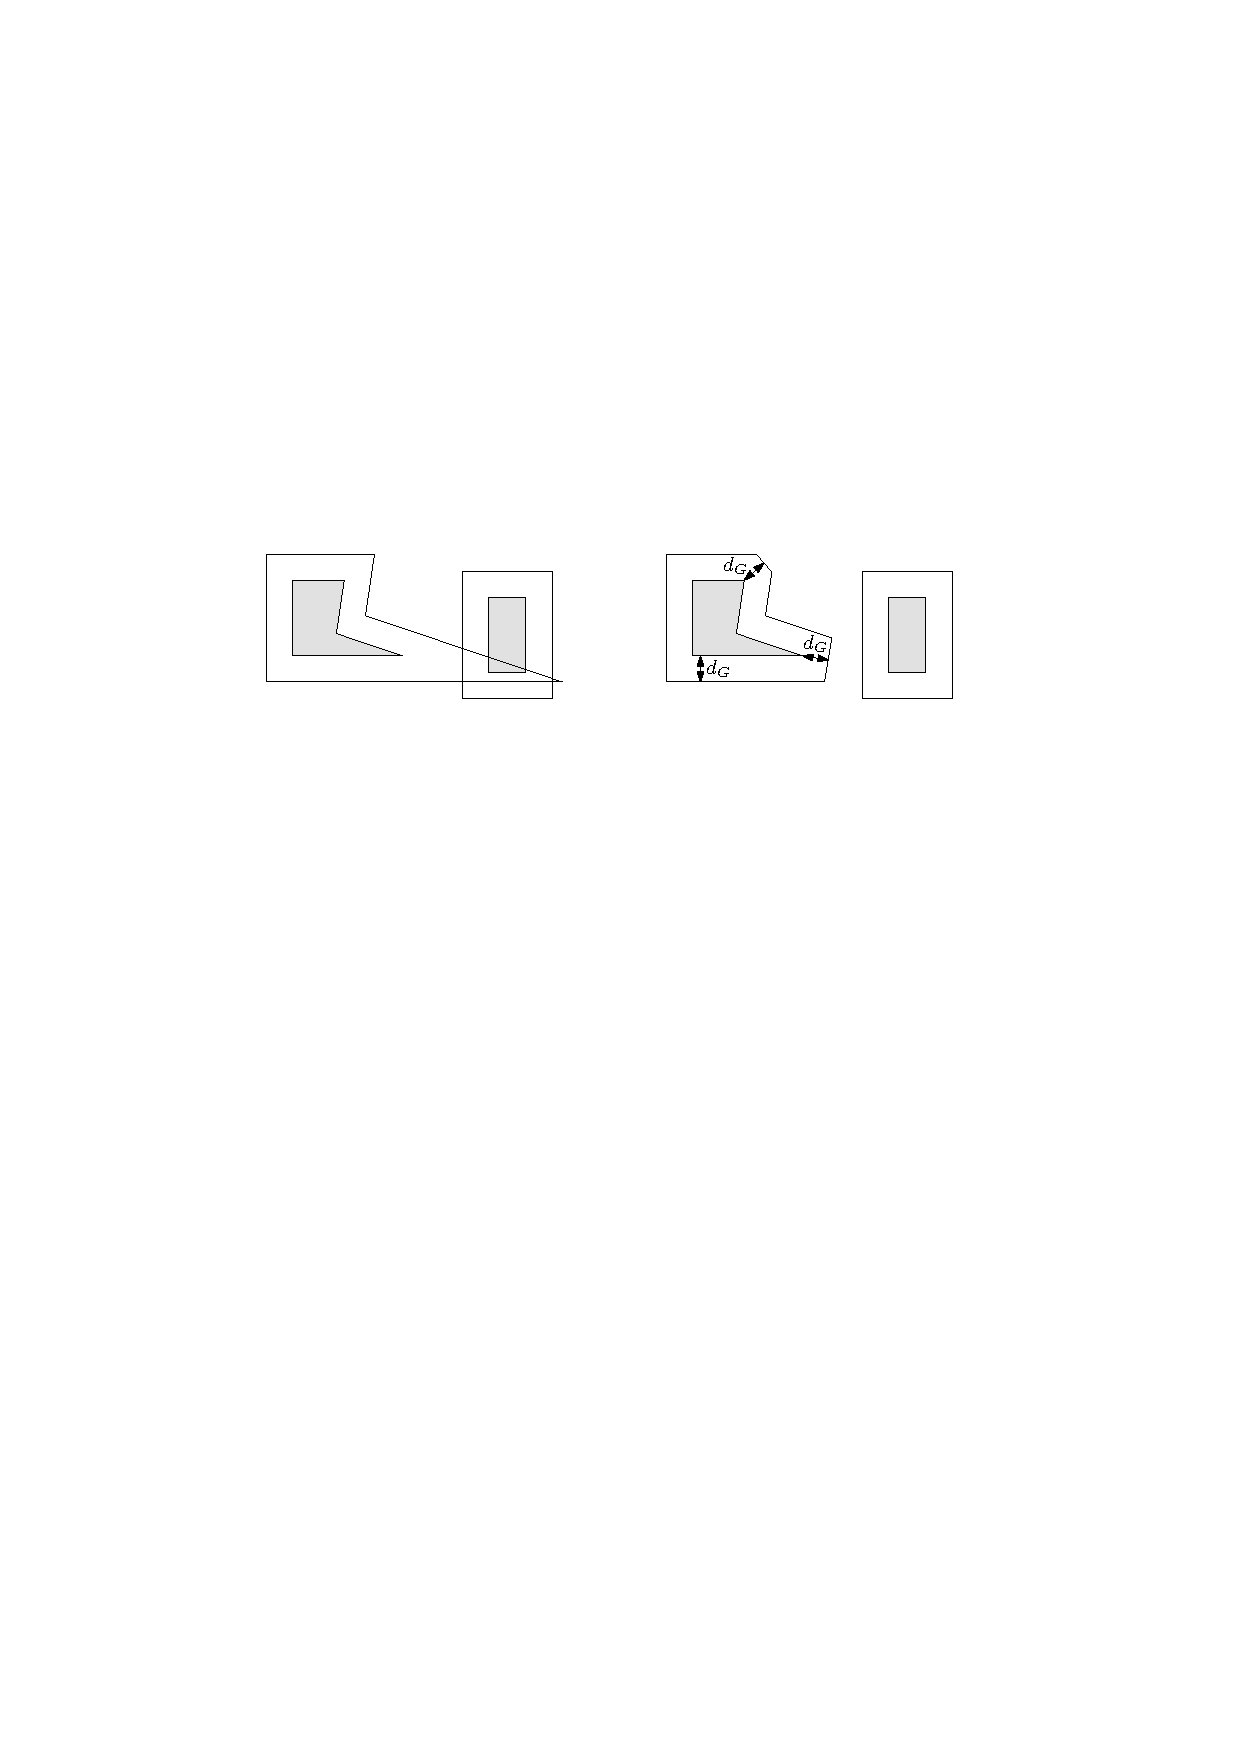
\includegraphics{Buffer_MiterLimits}
	\caption{}
	\label{fig:Buffer_MiterLimits}
\end{figure}


We denote by $d_\mathrm{G}$ the total growth. The growth at time $t$ is
\begin{equation}
	\label{eq:d_Gt}
	\dtrm{G} = t \cdot d_\mathrm{G}.
\end{equation}

\subsection{Simplifying grown buildings}
\label{sec:Simplify}
We use a buffering-based method, 
similar to \citet{Damen2008,Meijers2016}, 
to simplify our grown buildings. 
We first dilate the grown buildings to remove 
pits, and then erode the results to remove spikes
(see \fig\ref{fig:RemovePitAndSpike}).

\begin{figure}[tb]
	\centering
	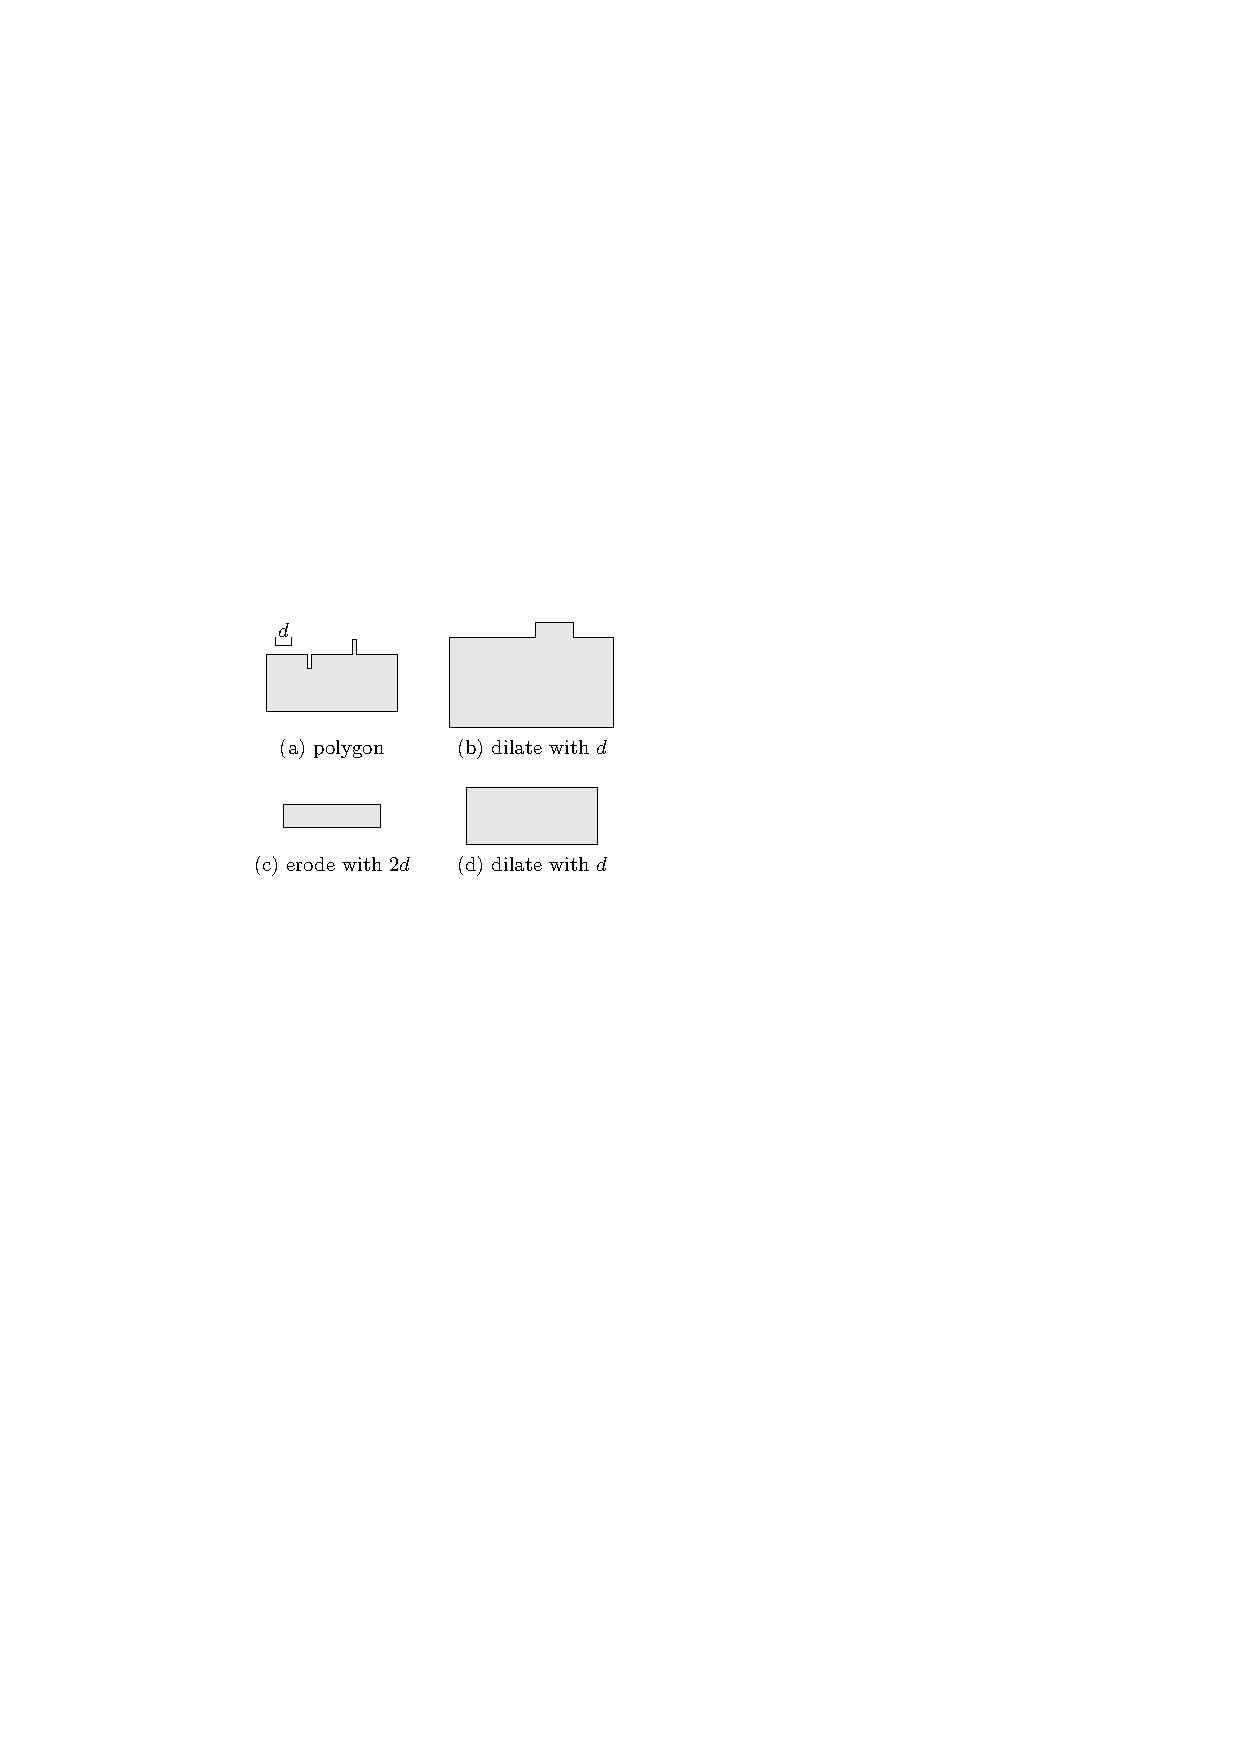
\includegraphics[]{RemovePitAndSpike}
	\caption{Remove a pit by dilating and then remove a spike by eroding.
		(a) a polygon with a pit and a spike;
		(b) dilate the polygon in (a) with distance $d$ to remove the pit;
		(c) erode the polygon in (b) with distance $2d$ to remove the spike;
		(d) dilate the polygon in (c) with distance $d$ so that the result has 
		the same size as the polygon in (a).
	}
	\label{fig:RemovePitAndSpike}
\end{figure}

At time $t$, we grow buildings with distance $\dtrm{G}$,
dilate with distance $\dtrm{D} (\dtrm{D}>0)$,
erode with distance $\dtrm{D}+\dtrm{E} (\dtrm{E}>0)$,
and dilate back with distance $\dtrm{E}$.
A problem we may have is that we may break a building by eroding.
The reason is that 
some parts of a building may be increased (by growing and dilating) 
with distance $\dtrm{G}+\dtrm{D}$, 
but be decreased (by eroding) as much as $\alpha (\dtrm{D}+\dtrm{E})$.
If  $\dtrm{G}+\dtrm{D} < \alpha (\dtrm{D}+\dtrm{E})$ 
and a building is not thick enough, 
the building may be broken into several parts
(see \fig\ref{fig:ErosionBreak}).
In order to avoid this problem, we require that
\[
\dtrm{G} + \dtrm{D} \ge \alpha (\dtrm{D}+\dtrm{E}),
\]
which means
\begin{equation}
\label{eq:d_Dt}
\dtrm{D} \le \frac{\dtrm{G}-\dtrm{E}}{\alpha - 1}.
\end{equation}

\begin{figure}[tb]
	\centering
	
\includegraphics[]{ErosionBreak}
	\caption{Dilate the gray polygon, then erode the dilated polygon.
		(a) Dilate and erode with distance $d_1$.
		(b) Dilate and erode with distance $d_2$, where $d_2>d_1$.
		In (a) the result of dilation and erosion is the same as the original 
		polygon, while in (b) the result consists of two parts.
	}
	\label{fig:ErosionBreak}
\end{figure}

We would like to use $\dtrm{E}=\frac{l}{2} \cdot M_t$
(see \eq\ref{eq:d_epsilont}) so that
any pits and spikes narrower than $l$ will be removed. 
We set $l=0.3\,\mathrm{mm}$, which was used as a length threshold by 
\citet{Regnauld2001,Li2004,Basaraner2008}.
Distance $\dtrm{G}$ can be arbitrarily small according to \eq\ref{eq:d_Gt}, 
but $\dtrm{E}$ is at least $\frac{l}{2} M_\mathrm{s}$. 
In this case, $\dtrm{G}-\dtrm{E} \le 0$ when $t$ is small, 
which violates \eq\ref{eq:d_Dt}, where $\dtrm{D}>0$.
As a compromise, we use
\begin{equation}
\label{eq:d_Et}
\dtrm{E} =t \cdot \frac{l}{2} M_\mathrm{g}.
\end{equation}
Still, we should make sure that $\dtrm{G}-\dtrm{E} > 0$, which means
$t \cdot \frac{\lambda}{2}\sqrt{a} (M_\mathrm{g}-M_\mathrm{s})-
t \cdot \frac{l}{2} M_\mathrm{g} >0$.
As a result, we should make sure that
\begin{equation}
\label{eq:S_g}
M_\mathrm{g} > \frac{\lambda\sqrt{a}}{\lambda\sqrt{a}-l} S_s.
\end{equation}

We wish to remove ``bays'' which have ``widths'' less than $2\sqrt{a_h/\pi}$.
\todo{why? more details}
Usually, our $\dtrm{D}$ is not large enough to do so.
We use the upper bound in \eq\ref{eq:d_Dt}, that is,
\[
\dtrm{D} = \frac{\dtrm{G}-\dtrm{E}}{\alpha - 1}.
\]

After carrying out the buffering-based methods, 
we simplify the grown buildings using Imai--Iri algorithm 
\citep{ImaiIri1988}.
This algorithm first finds all the valid shortcuts of a polyline.
A shortcut is valid for a segment 
if the distance between the segment and the shortcut is at most a specified 
value
(see \fig\ref{fig:ImaiIri_Shortcut}).
We set the value also as $l$.
That is, at time $t$, the threshold distance is
\begin{equation}
\label{eq:d_lt}
d_{l,t}= l \cdot M_t.
\end{equation}
Second, the algorithm finds a sequence of valid shortcuts, from the beginning 
of a polyline to the end, using breadth-first search.
The sequence of valid shortcuts is an approximation of the polyline, 
and has the least number of line segments.

\begin{figure}[tb]
	\centering
	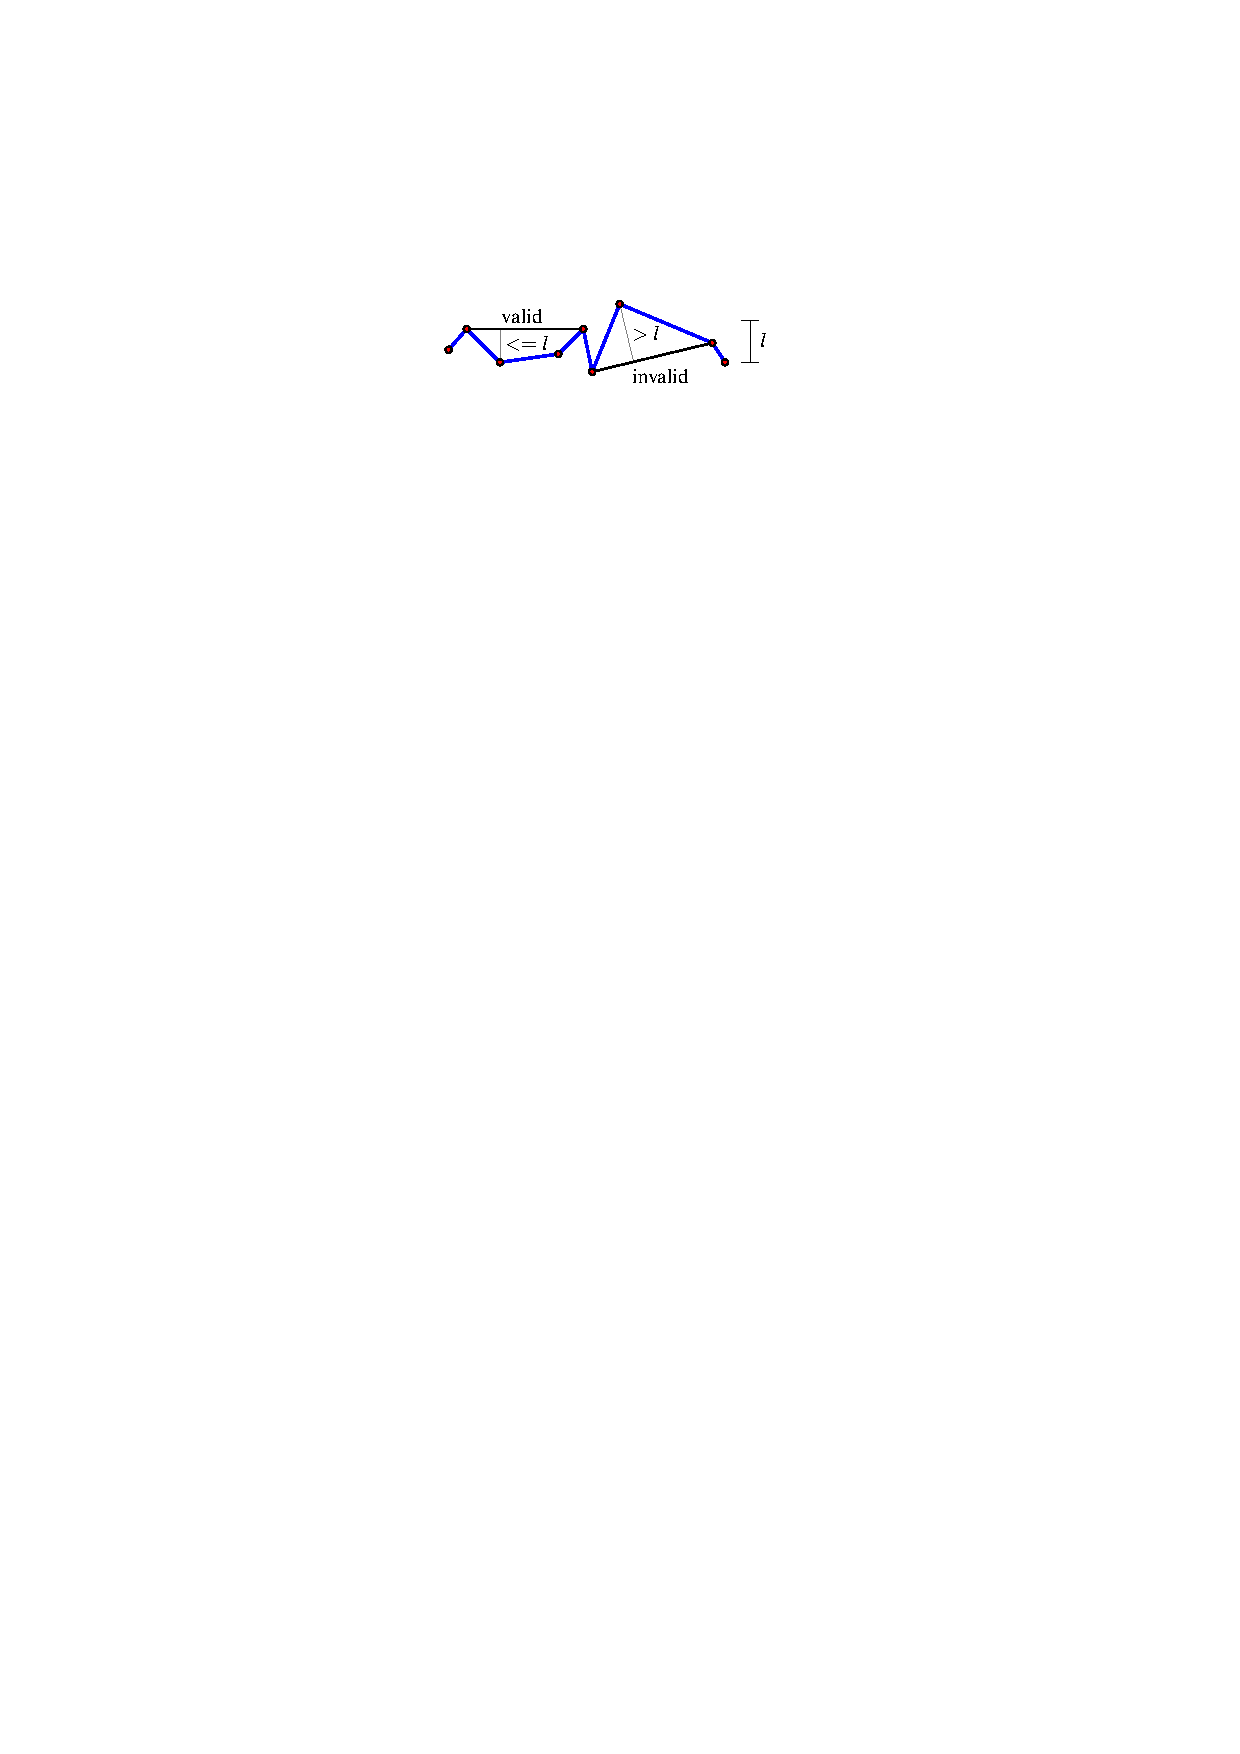
\includegraphics[]{ImaiIri_Shortcut}
	\caption{Valid and invalid shortcuts for Imai--Iri algorithm.}
	\label{fig:ImaiIri_Shortcut}
\end{figure}

\todo[inline]{more details in the below paragraph?}
We add two more constraints for a shortcut to be valid. 
First, a shortcut must be completely inside the grown building.
If a shortcut is outside,
we are not able to arrive at the shortcut by growing.
Second, a shortcut is not allowed to intersect the 
boundary of the original building.
If we allow this intersection, 
we need to shrink the building instead of growing. 
Of course, we do not want to shrink.

We tried simplifying using 
the Douglas--Peucker algorithm \citep{Douglas1973}, 
but we hoped to remove more points. 
We found that the Imai--Iri 
algorithm fit our needs better. 






\subsection{Generating the goal forms of buildings}
\label{sec:Goal}
To generate the goal forms of buildings, we set time $t=1$.
We group (see \sect\ref{sec:Group}) 
and merge (see \sect\ref{sec:Merge}) buildings on start map.
Then we grow (see \sect\ref{sec:Grow}) 
and simplify (see \sect\ref{sec:Simplify}) the merged buildings.
See for example \fig\ref{fig:Buffer_MiterLimits}, 
the building at time $t=1$ is the goal form of the three buildings of $t=0$.




\subsection{Generating buildings on intermediate-scale maps}
\label{sec:Unite}

Both the erosion and line simplification may results in shrinking of a 
building.
\fig\ref{fig:Shrink_Erosion} and \fig\ref{fig:Shrink_Simplification} show such 
examples respectively.
To avoid these kinds of shrinking,
we unite a building with itself at the immediately previous step.
For example, if the grown polygons of 
\fig\ref{fig:Shrink_Erosion}~(c) and~(g) 
are from a sequence of $10$ steps, 
i.e., $t \in \{0.1, 0.2, \dots, 1\}$, 
then we compute the result of $t=0.8$ by uniting 
the grown polygon obtained independently at $t=0.8$ and 
the grown polygon at $t=0.7$. 
\fig\ref{fig:Shrink_Uniting}~(a) shows the result,
which is the union of the two grown polygons in 
\fig\ref{fig:Shrink_Erosion}~(c) and~(g).
Similarly, \fig\ref{fig:Shrink_Uniting}~(b) shows the union of the two grown 
polygons in 
\fig\ref{fig:Shrink_Simplification}~(c) and~(h).

A building on an intermediate map should never exceed
the goal form of the group of buildings 
which include the united buildings. 
Otherwise, the building will need to be shrunk.
To guarantee the non-exceeding, 
we clip the building by the goal form 
and remove the parts outside.
\todo{example?}

\begin{figure*}[tb]
	\centering
	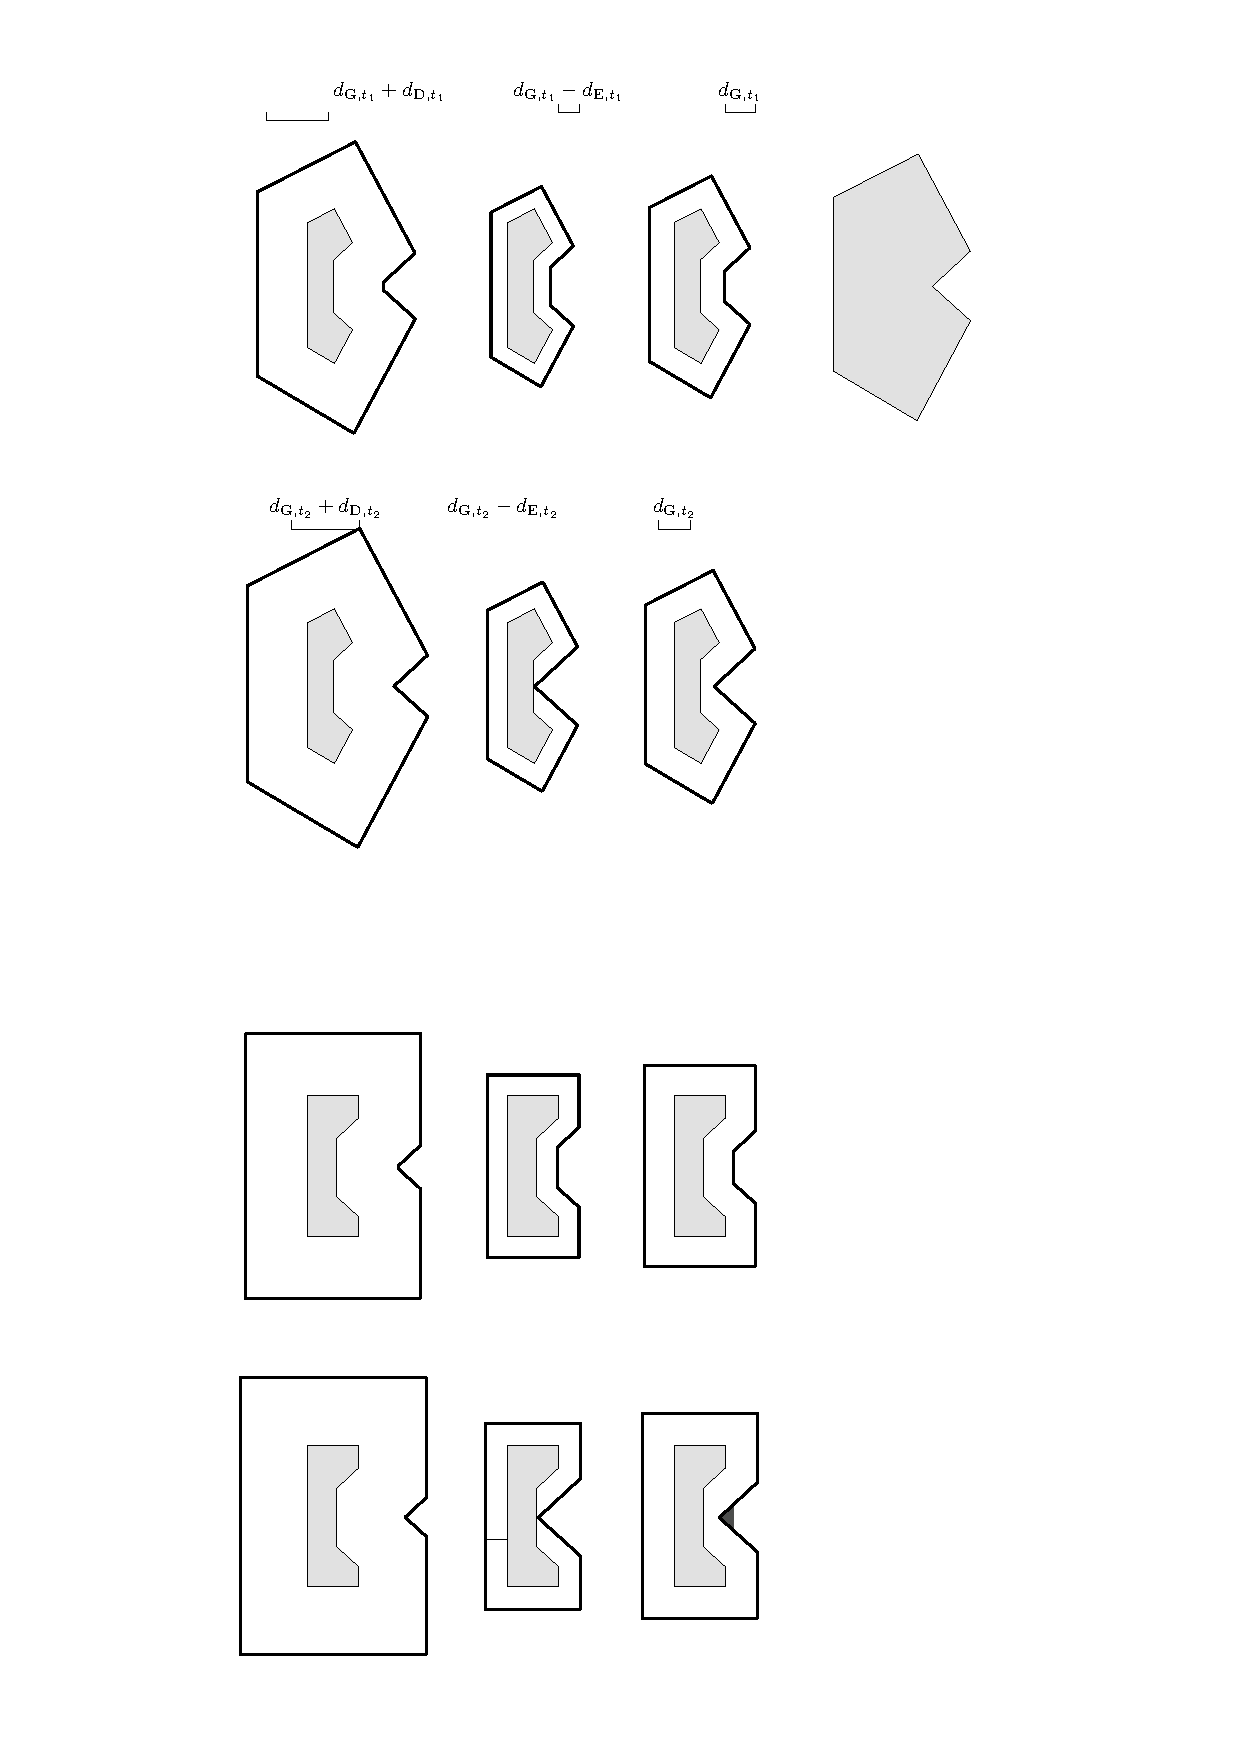
\includegraphics[]{Shrink_Erosion}
	\caption{A building shrinks during growing because of dilation and erosion, 
		where $t_1=0.6$, $t_2=0.7$, and $t_3=1$.
		The small gray polygons represent the original building.
		(a) Grow and Dilate the building with distances $\dtrm[1]{G}$ and 
		$\dtrm[1]{D}$, respectively;
		(b) Erode the polygon in (a) with distance $\dtrm[1]{D} + \dtrm[1]{E}$;
		(c) Dilate the polygon in (b) with distance $\dtrm[1]{E}$.
		(d) The large gray polygon is the target shape on goal map.
		The process for (e), (f), and (g) is the same as the process of (a), 
		(b), and (c).
		The darker gray piece in (g) shows 
		the part which is included in the grown polygon of (c), 
		but not in the grown polygon of (g).
	}
	\label{fig:Shrink_Erosion}
\end{figure*}

\begin{figure*}[tb]
	\centering
	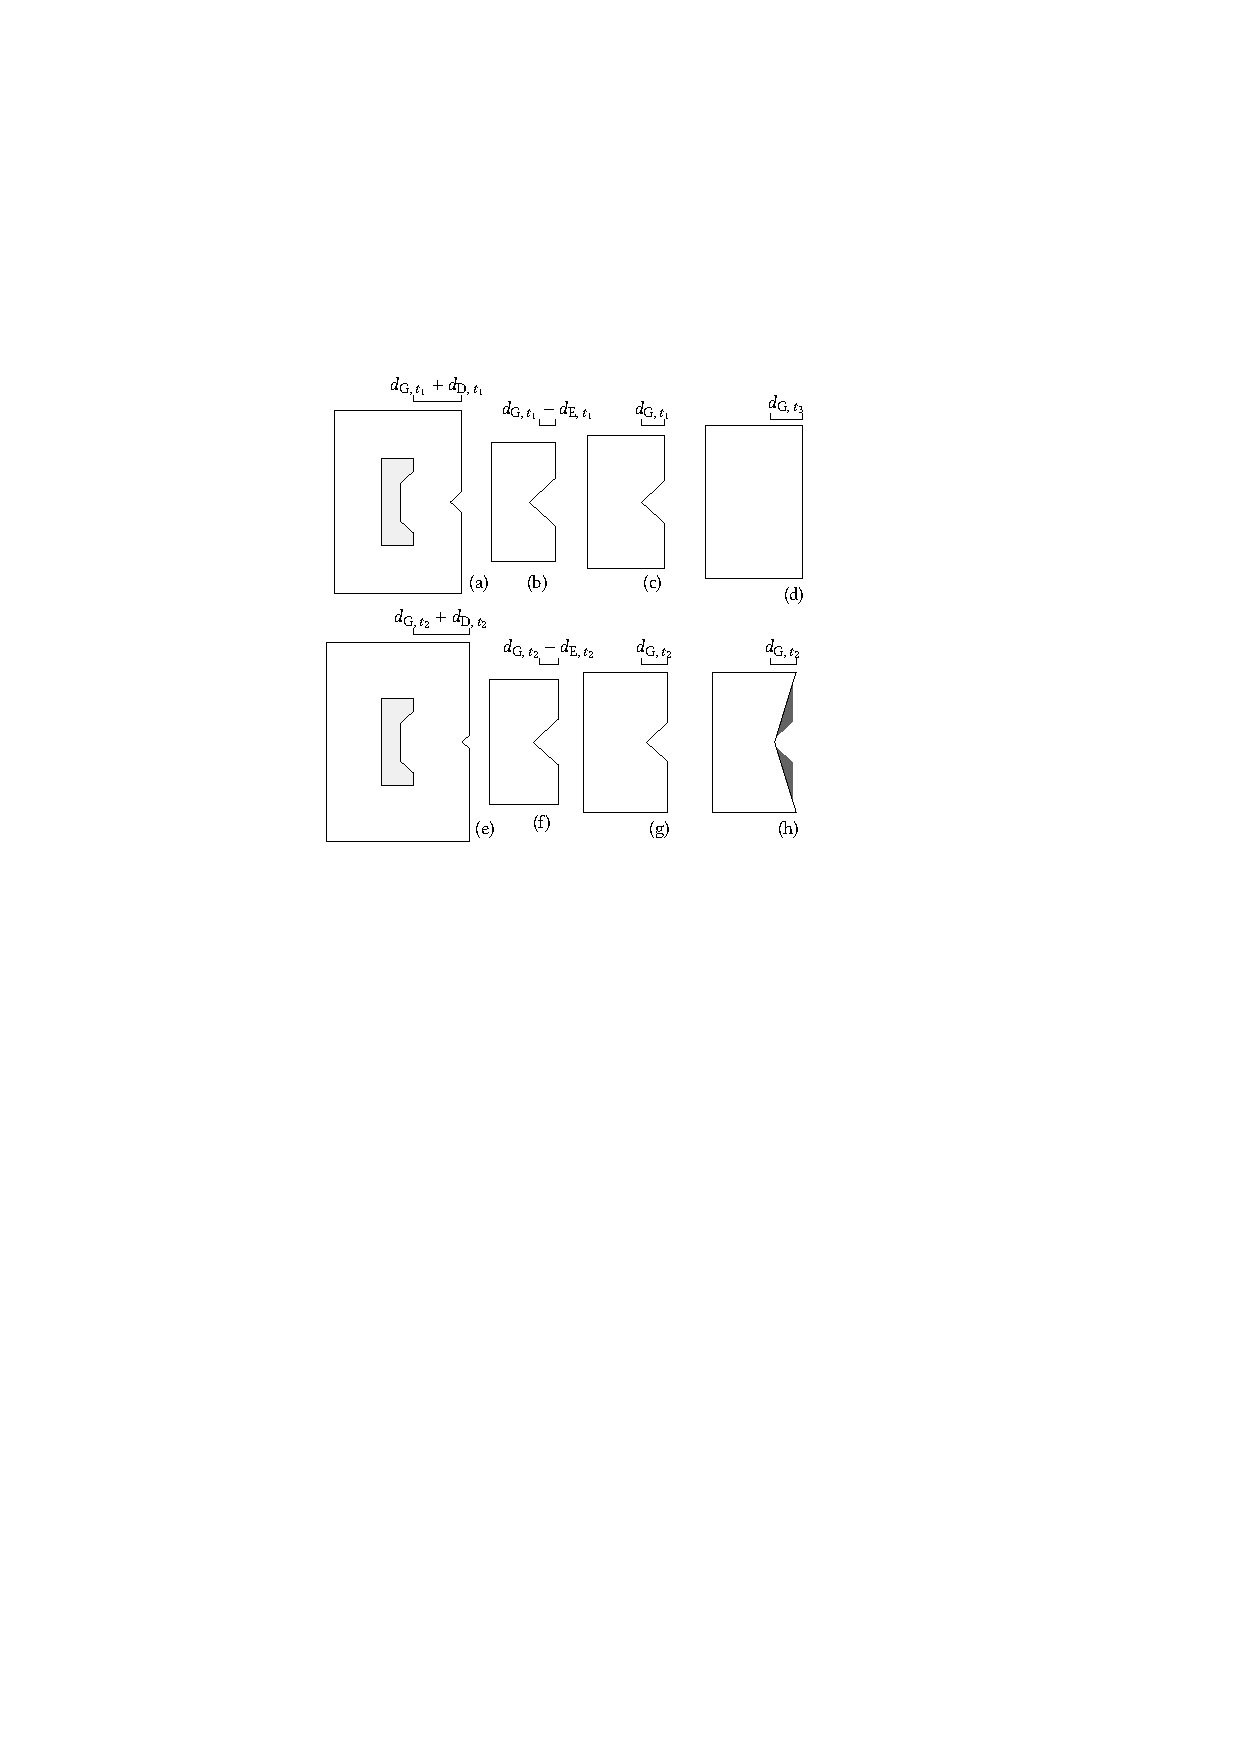
\includegraphics[]{Shrink_Simplification}
	\caption{A building shrinks during growing because of line simplification, 
		where $t_1=0.7$, $t_2=0.8$, and $t_3=1$.
		The small gray polygons represent the original building.
		The process for (a), (b), and (c), and 
		the process for (e), (f), and (g) are the same as 
		the processes in \fig\ref{fig:Shrink_Erosion}.
		(d) The large gray polygon is the target shape on goal map.
		(h) Simplify the polygon in (g) using the Imai--Iri algorithm.
		Note that $d_{l,t_1}<d_{l,t_2}$ see \eq\ref{eq:d_lt}),
		which is why the Imai--Iri algorithm does not 
		remove any point of the polygon in (c),
		but removes two points of the polygon in (g).
		The darker gray pieces in (h) show 
		the parts which are included in the polygon of (c), 
		but not in the polygon of (h).
	}
	\label{fig:Shrink_Simplification}
\end{figure*}

\begin{figure}[tb]
	\centering
	
\includegraphics[]{Shrink_Uniting}
	\caption{Unite a polygon with the polygon at the immediately previous step.
		(a) Unite the polygon of \fig\ref{fig:Shrink_Erosion}c and the 
		polygon of \fig\ref{fig:Shrink_Erosion}g;
		(b) Unite the polygon of \fig\ref{fig:Shrink_Simplification}c and 
		the polygon of \fig\ref{fig:Shrink_Simplification}h;
	}
	\label{fig:Shrink_Uniting}
\end{figure}




\subsection{Eliminating small buildings}
\label{sec:Eliminate}
We eliminate a building if the area of this building is smaller than a 
threshold.
For a group of buildings, we consider the area sum of all the buildings.


%\subsection{Parameters for growing and simplifying}
%
%
%
%
%If we insist on that we should observe 
%the growing, say, $x \% (0<x<100)$ of the time at least, then we should make 
%sure that
%\begin{equation}
%\label{eq:a_limit}
%\frac{d_\mathrm{G}}{d_\mathrm{G}+d_\epsilon} \ge x \%.
%\end{equation}
%Using $d_\mathrm{G}$ and $d_\epsilon$ from Eqs.~\ref{eq:d_G} 
%and~\ref{eq:d_epsilon}, we transform Eq.~\ref{eq:a_limit} to
%\begin{equation}
%a \ge \Big(\frac{2 \epsilon S_g x}{\lambda (100-x) (S_g-S_s)}\Big)^2
%\end{equation}
%We also require 
%that $S_g \ge 2 S_s$, which means $S_s \le \frac{1}{2} S_g$.
%On one hand, we should have a large $x$ so that we will see the 
%growing most of the time.
%On the other hand, we wish to keep bridges short as bridges are intrusions to 
%our map, which means we should have a small $x$ and a large $\lambda$ so that 
%we will have a small 
%$a$ (according to Eq.~\ref{eq:a_limit}), a small $d_\mathrm{G}$ (according to 
%Eq.~\ref{eq:d_G}), and finally a small $l_b$ (according to 
%Eq.~\ref{eq:BridgeLength}). Also we should have a small $x$ and a large 
%$\lambda$ as our $a$ is already much larger than $0.16\,\mathrm{mm}^2$ on 
%map, which is the area limit used by \citet{Stoter2009}. As a result, we 
%set 
%$\lambda=0.8$ and $x=\frac{2}{3} \cdot 100$.
%Using these setting, we have
%\begin{equation}
%a \ge 4.
%\end{equation}
%according to Eq.~\ref{eq:a_limit}.
%
%
%
%
%Therefore, we may grow up to distance 
%\[
%D_\mathrm{G} = d_\mathrm{G} + d_\epsilon.
%\]
%Fig.~\ref{fig:ExtraGrowth} shows such an enlargement and simplification, 
%where  
%variable $d_\mathrm{e} (\le d_\epsilon)$ is the extra growing distance.
%
%
%\citet{Chaudhry2008} thought that a hole of a settlement should be at least 
%$0.5\,\mathrm{km}^2$ for a map at scale $1:250{,}000$, 
%which means that the hole is at least $8\,\mathrm{mm}^2$ on map. 
%Following their setting, we shrink a hole and 
%eliminate the hole once its size is smaller than $8\,\mathrm{mm}^2$ on map.







%
%A hole has area less than $\pi D_\mathrm{G}^2$ can be filled by growing. 
%A hole has area 
%slightly more than $\pi D_\mathrm{G}^2$ will become a very small hole after 
%growing with 
%distance $D_\mathrm{G}$. In order to avoid small holes, we do not fill a hole 
%unless the 
%area of the hole on the start map is smaller than $\pi D_\mathrm{G}^2$. Note 
%that we do 
%not fill a hole even if the hole has a large area because a large hole may be 
%split into several small holes by filling. 
%Although our intermediate results may violate the rule that a hole should be 
%at 
%least some size, we try to avoid the violation for a map at a goal scale.
%\citet{Chaudhry2008} thought that a hole of a settlement should be at 
%least 
%$0.5$ km$^2$ for a map at scale $1:250{,}000$, which means that the hole is 
%at 
%least $8\,\mathrm{mm}^2$ on the map. Following their setting, we wish to have 
%$\pi 
%D_\mathrm{G}^2 \ge 8 S_g^2$.
%
%
%Now we discuss how to set the parameters according to our requirements. 
%First, 
%we wish to increase $d_\mathrm{G}/d_\epsilon$. Most part of a building will 
%grow $d_\mathrm{G}$. Only a small part will continue growing after the 
%building 
%has grown $d_\mathrm{G}$. To ensure that we can see the growing most of the 
%time, we want to have a large $d_\mathrm{G}/d_\epsilon$.
%
%
%
%
%
%We cannot fulfill all the requirements. 

%\begin{figure*}[tb]
%	\centering
%	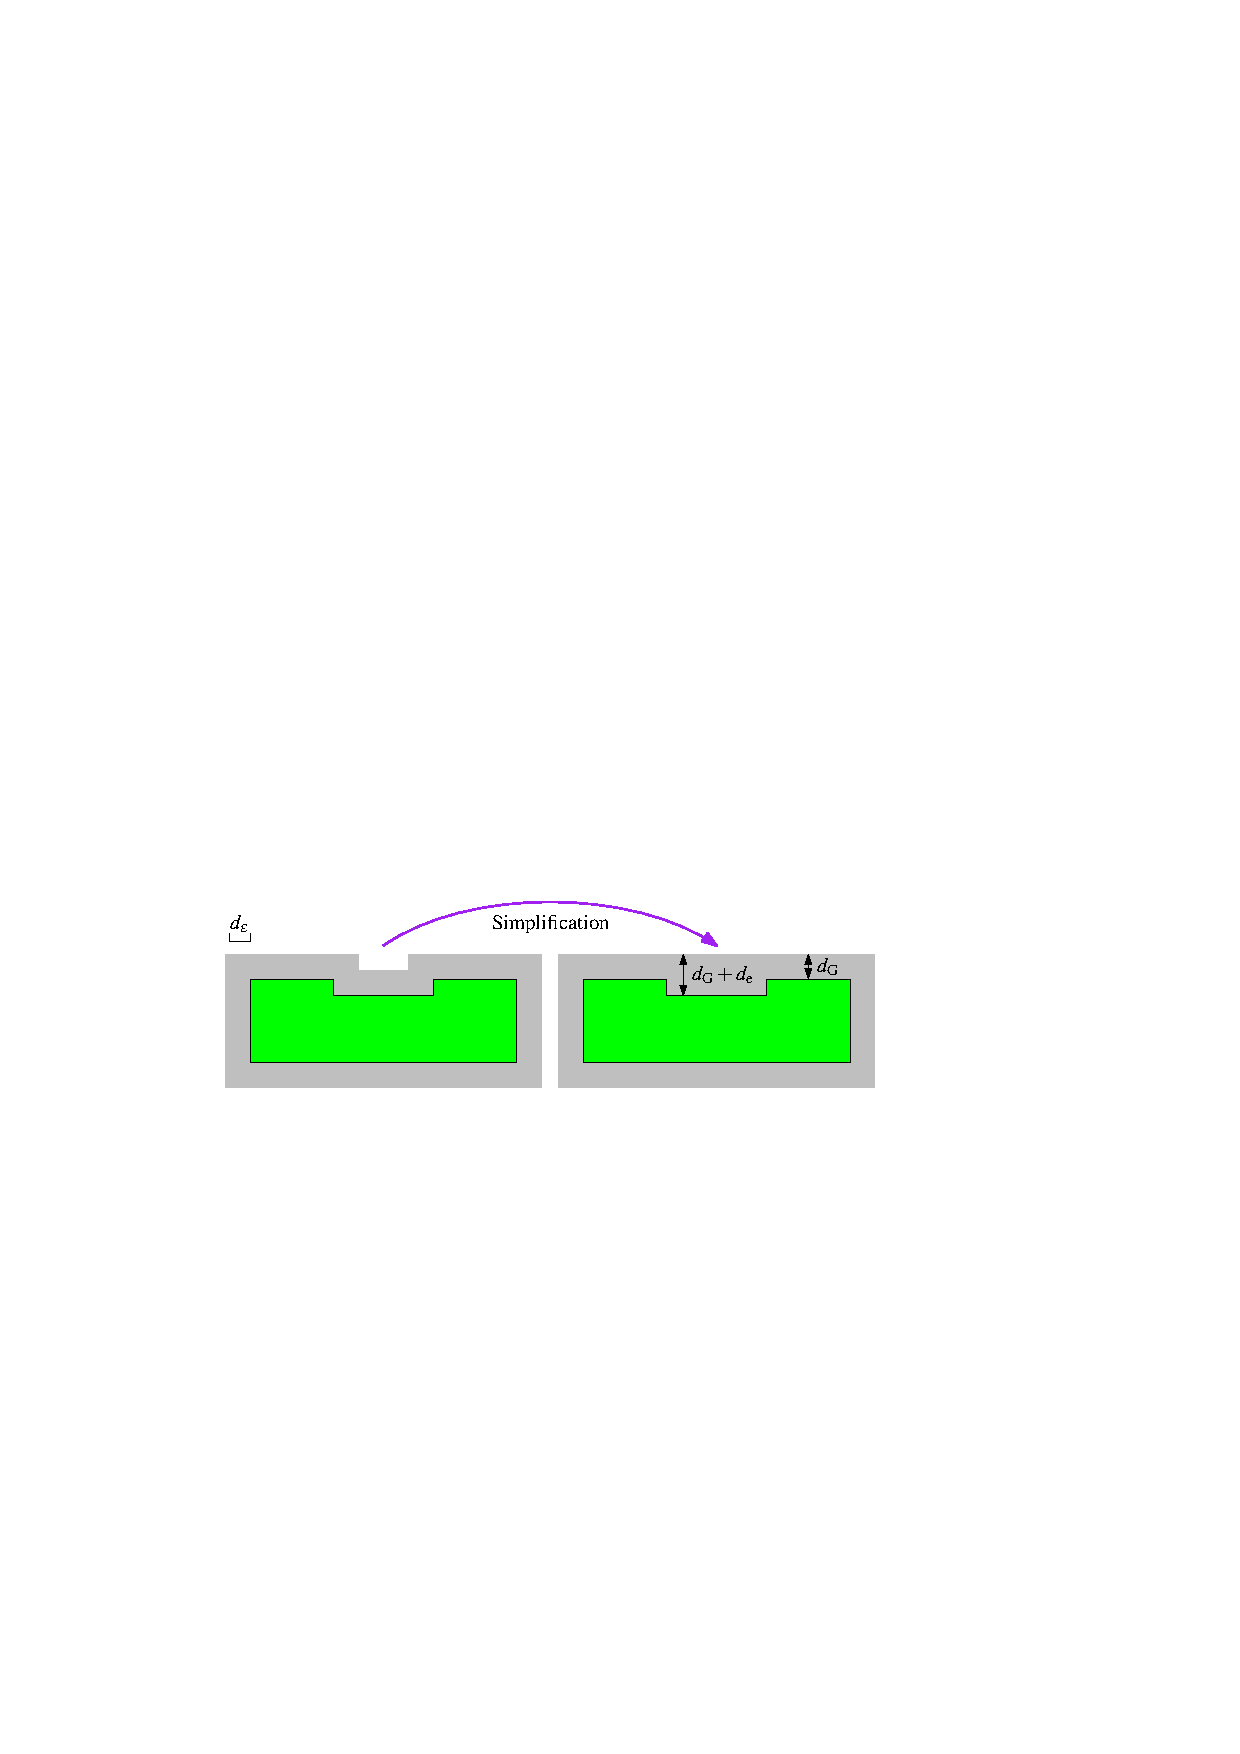
\includegraphics{ExtraGrowth}
%	\caption{In the left figure, the green polygon represents a building, and 
%		the gray polygon is the enlargement of the building. In the right 
%		figure, the gray polygon has been simplified to a rectangle. In order 
%to 
%		fill the rectangle, most parts of the (green) building needs to grow 
%with
%		distance $d_\mathrm{G}$, but the pit needs to grow with $d_G + 
%		d_\mathrm{e}$, 
%		where $d_\mathrm{e}$ is the extra growing distance.}
%	\label{fig:ExtraGrowth}
%\end{figure*}


%\begin{figure*}[tb]
%	\centering
%	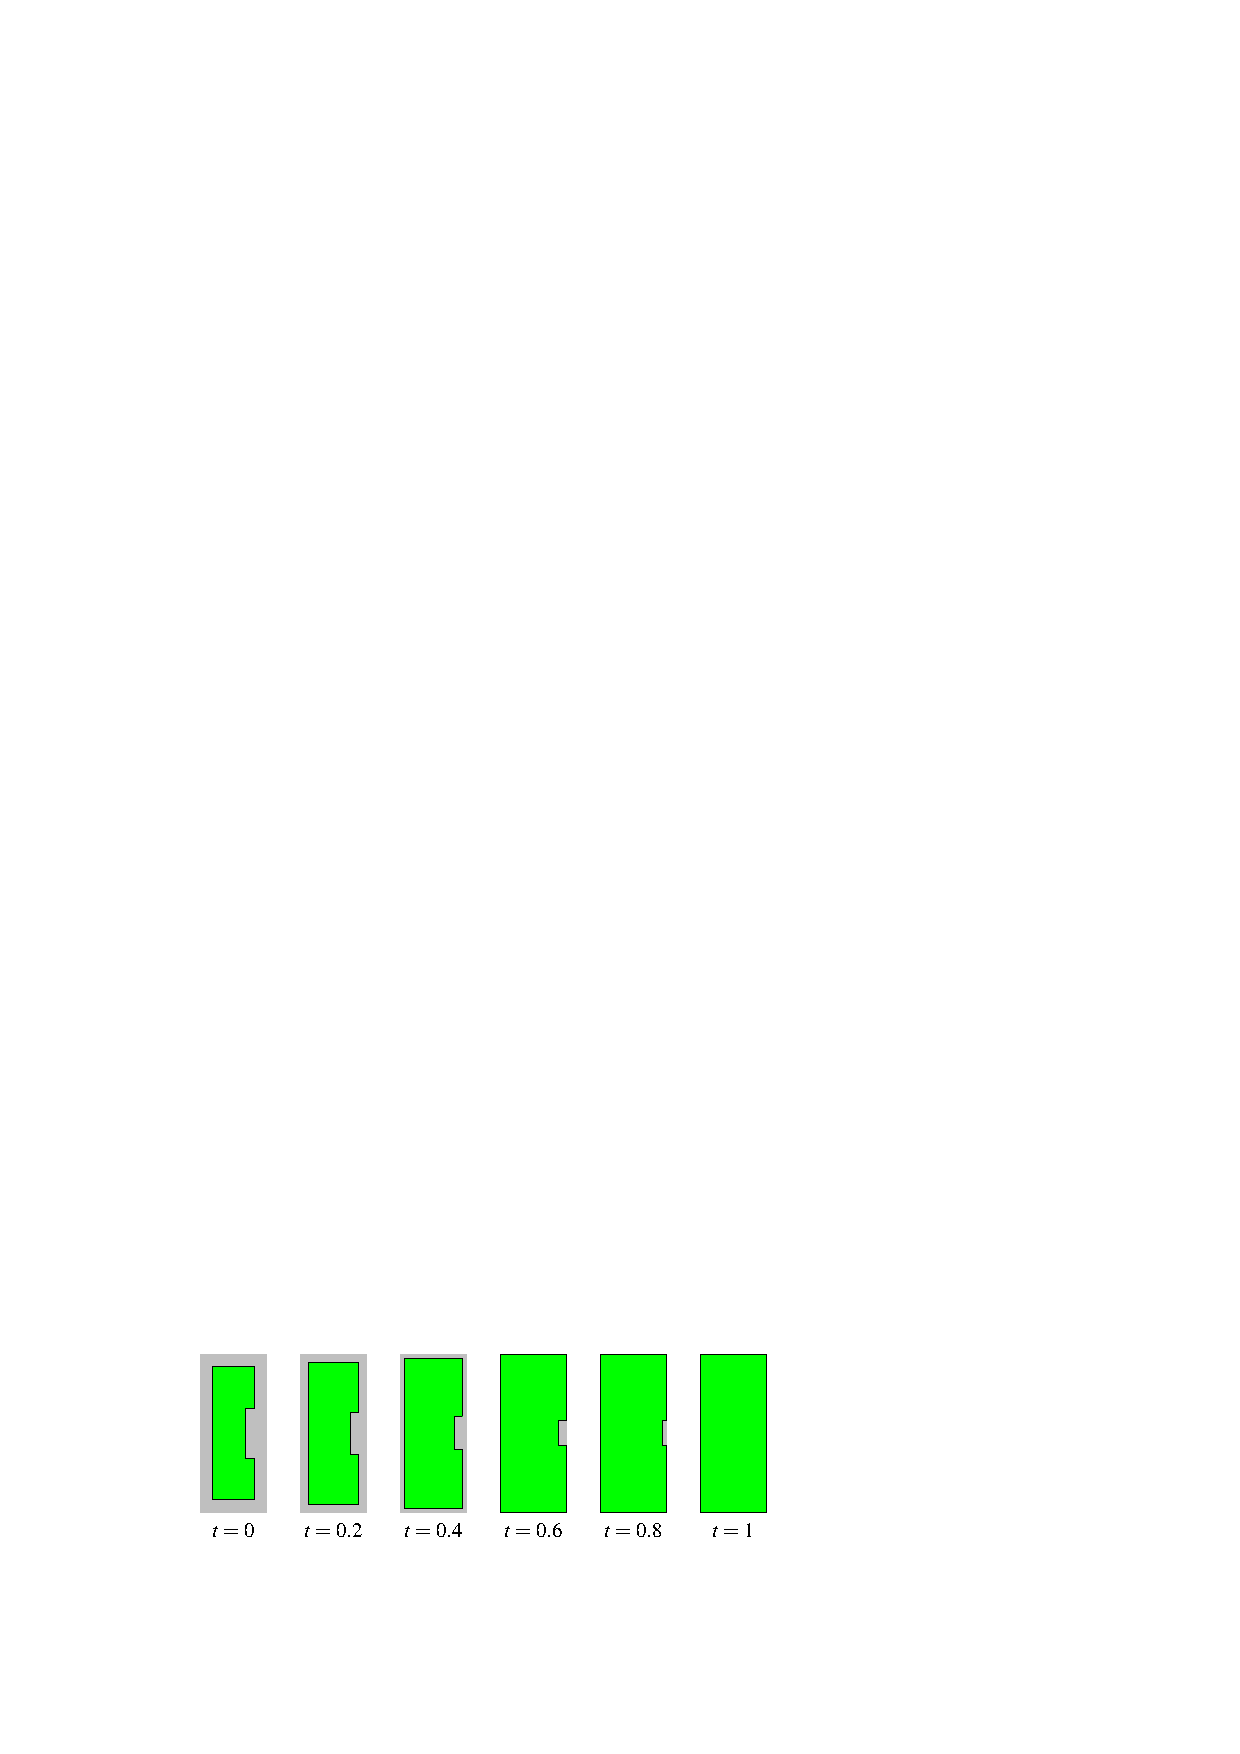
\includegraphics{GrowingExample}
%	\caption{GrowingExample.}
%	\label{fig:GrowingExample}
%\end{figure*}

%\subsection{Running time analysis}
%Although a version with a 
%lower running time exists \citep[see][]{Chan1992}, we implemented the basic 
%version.


\section{Case Study}
\label{sec:CaseStudy}
We have implemented our method based on
C\# (Microsoft Visual Studio 2015) and ArcObjects SDK 10.4.1.
The buffer function and clip function are from library \emph{Clipper} 
of \citet{Johnson2014}.
An evaluation of Clipper can be found in \citet{Palfrader2015}.
We ran our case study under 64-bit 
Windows 7 on a 3.3 GHz dual core CPU with 8 GB RAM.
We measured processing time by the built-in C\# class 
\emph{Stopwatch}.
We tested our method on a dataset from French Mapping Agency (IGN).
The dataset represents four towns (communes in French), i.e., Aussevielle, 
Denguin,  Poey-de-Lescar, and Siros, in the 
Pyr\'en\'ees-Atlantiques department, south-western France.
The scale of the dataset is $1:15{,}000$.
There are $2{,}590$ buildings (see \fig\ref{fig:Data}), 
which has $19{,}255$ edges in total.
Our goal scale is $1:50{,}000$.


\begin{figure*}[tb]
	\centering
	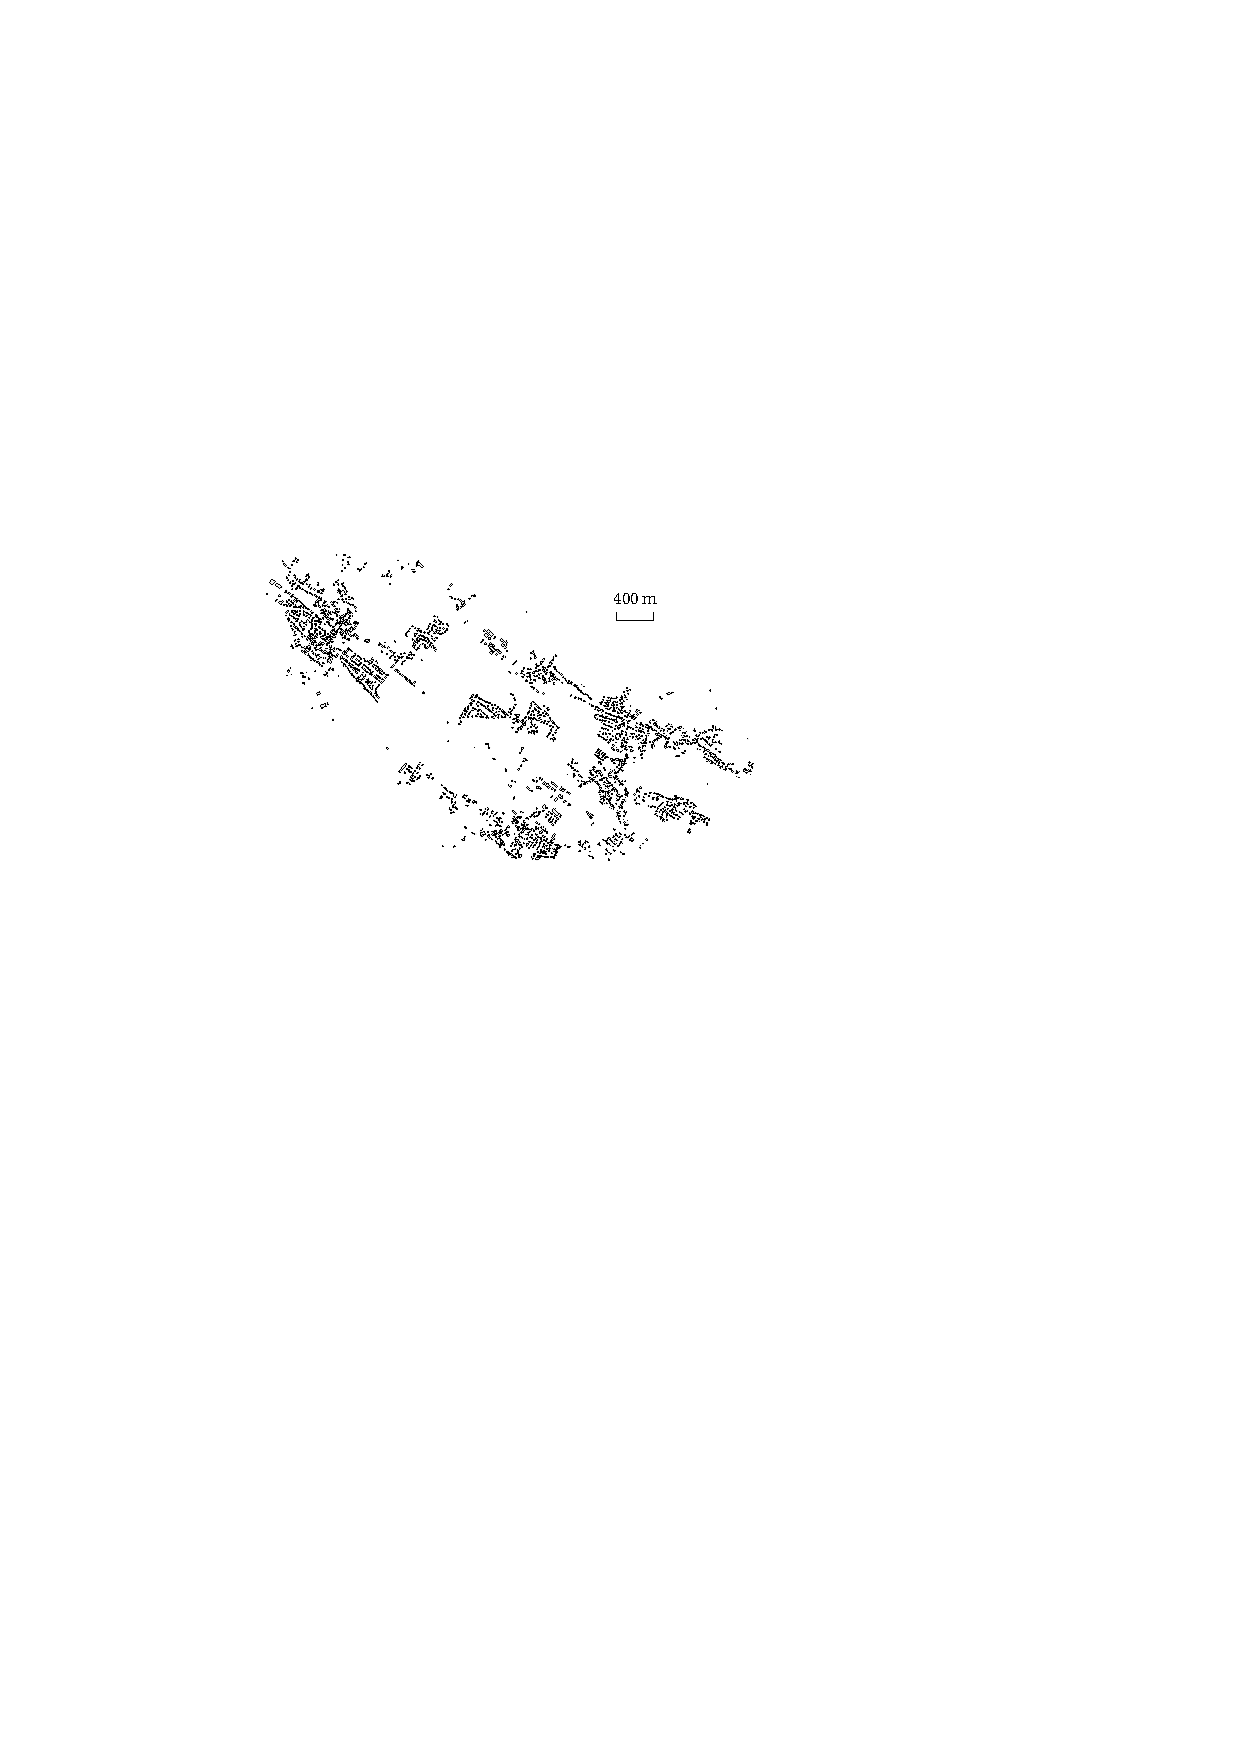
\includegraphics{Data}
	\caption{scale.}
	\label{fig:Data}
\end{figure*}

\todo[inline]{comparison of simplification between Douglas--Peucker and 
	Imai--Iri}


The area on start map is $some number\,\text{mm}^2$.
Our area on map is $some number\,\text{mm}^2$.
According to \eq4 of paper \citet{Topfer1966}, 
the area on map should be $some number\,\text{mm}^2$

%Although a version with a 
%lower running time exists \citep[see][]{Chan1992}, we implemented the basic 
%version

\section{Conclusion}
\label{sec:Conclusion}


Our intermediate results may violate more cartographic rules, but we try to 
make the results at goal scales violate as few rules as possible.


Eventually, our result is a set of settlement boundaries. An interesting 
problem is to compare our method with \citet{Chaudhry2008}.

We used radical law. We may also consider the fractal nature of maps proposed 
by \citet{Jiang2015}.

We did not include streets. We can either put them above the settlement 
boundaries on map, or use them as restriction for building growing.

Show some results obtained by ArcGIS.
Show the data at $1:50{,}000$.

A special kind of Voronoi diagram considering miter offset. A buildings is 
allowed to grow inside its own zone.

\todo[inline]{consider multi bridges; 
	consider transparency of bridges in stead of enlarging}